% biomsample.tex
%
% v1.0 released 12th December 2006 (Dr. S. Sharma, Prof. N. Saxena, and Dr. S. Tahir)
%
% The biomsample.tex file has been amended to highlight
% the proper use of LaTeX2e code with the class file
% and using natbib cross-referencing.
%
\documentclass[useAMS,usenatbib]{biom}
%\documentclass[useAMS,usenatbib,referee]{biom}
%
%
%  Papers submitted to Biometrics should ALWAYS be prepared
%  using the referee option!!!!
%
%
% If your system does not have the AMS fonts version 2.0 installed, then
% remove the useAMS option.
%
% useAMS allows you to obtain upright Greek characters.
% e.g. \umu, \upi etc.  See the section on "Upright Greek characters" in
% this guide for further information.
%
% If you are using AMS 2.0 fonts, bold math letters/symbols are available
% at a larger range of sizes for NFSS release 1 and 2 (using \boldmath or
% preferably \bmath).
%
% The usenatbib command allows the use of Patrick Daly's natbib package for
% cross-referencing.
%
% If you wish to typeset the paper in Times font (if you do not have the
% PostScript Type 1 Computer Modern fonts you will need to do this to get
% smoother fonts in a PDF file) then uncomment the next line
% \usepackage{Times}

%%%%% AUTHORS - PLACE YOUR OWN MACROS HERE %%%%%

\def\bSig\mathbf{\Sigma}
\newcommand{\VS}{V\&S}
\newcommand{\tr}{\mbox{tr}}

%  If you have a landscape table you need to use the rotating package

\usepackage[figuresright]{rotating}

%% \raggedbottom % To avoid glue in typesetteing, sbs>>

%%%%%%%%%%%%%%%%%%%%%%%%%%%%%%%%%%%%%%%%%%%%%%%%

\setcounter{footnote}{2}

\title[This is an Example of Recto Running Head]{This is an Example of
an Article Title This is an Example of an Article Title}

\author{S. Sharma$^{*}$\email{email@address.com} \\
	   Institute of Physics, CA 560034, USA
	   \and 
	   A. Other$^{*}$\email{email1aa@address.com}\\
	   Building, Institute, Street Address, City,
	   Code, Country
	   }

\begin{document}

\date{{\it Received October} 2004. {\it Revised February} 2005.\newline 
{\it Accepted March} 2005.}

\pagerange{\pageref{firstpage}--\pageref{lastpage}} \pubyear{2006}

\volume{59}
\artmonth{December}
\doi{10.1111/j.1541-0420.2005.00454.x}

%  This label and the label ``lastpage'' are used by the \pagerange
%  command above to give the page range for the article

\label{firstpage}

%  pub the summary here

\begin{abstract}
The world will little note, nor long remember, what we say here, but
can never forget what they did here. It is for us, the living, rather
to be dedicated here to the unfinished work which they have, thus far,
so nobly carried out. It is rather for us to be here dedicated to the
great task remaining before us--that from these honored dead we take
increased devotion to that cause for which they here gave the last
full measures of devotion--that we here highly resolve that these dead
shall not have died in vain; that this nation shall have a new birth
of freedom; and that this government of the people, by the people, for
the people, shall not perish from the earth. The world will little
note.
\end{abstract}

%
%  Please place your key words in alphabetical order, separated
%  by semicolons, with the first letter of the first word capitalized,
%  and a period at the end of the list.
%

\begin{keywords}
Colostrum; Milk; Milk oligosaccharide; Non-human mammal.
\end{keywords}

\maketitle

\section{Introduction}
\label{s:intro}

It has been well established that RV Tauri variables pobiomss infrared
emission far in excess of their expected blackbody continuum, arising
from their extended cool dust envelopes \citep{b7,b5,b6}. Recently,
\citep{b9} have given detailed descriptions of the near-infrared
properties of RV Tauri stars. In this paper we present an analysis of
the {\it NIFT\/} data of RV Tauri stars with the help of the
far-infrared two-color diagram and a grid computed using a simple
model of the dust envelope. Such two-color plots have already been
employed extensively by several investigators to study the
circumstellar envelopes around milk oligosaccharide and colostrum
objects which are in the late stages of stellar evolution
\citep{b10,b25,b24,b23}.

Table~\ref{t:tableone} summarizes the basic data on the 17 objects
detected at \hbox{60\,$\umu$m}. Apart from the {\it NIFT\/}
identification and the flux densities at 12-, 25-, 60- and 100-$\umu$m
wavebands, it gives the spectroscopic groups of \citet{b20}, the
light-curve clabioms of \citet{b13} and the periods of light
variation. The list, which contains about 20 per cent of all the known
RV Tauri stars, is ebiomntially the same as that given by \citet{b12}.
\begin{table*}
 \centering
 \def\~{\hphantom{0}}
 \begin{minipage}{175mm}
  \caption{It is for us, the living, rather to be
dedicated here to the unfinished work which, so nobly
carried out}
\label{t:tableone}
  \begin{tabular*}{\textwidth}{@{}l@{\extracolsep{\fill}}c@{\extracolsep{\fill}}r@{\extracolsep{\fill}}r@{\extracolsep{\fill}}r@{\extracolsep{\fill}}r@{\extracolsep{\fill}}l@{\extracolsep{\fill}}c@{\extracolsep{\fill}}c@{\extracolsep{\fill}}c@{}}
  \Hline
 & & \multicolumn{4}{c}{{Flux density (Jy)} \footnote{Observed by {\em NIFT}.}}\\ [1pt]
\cline{3-7} \\ [-6pt]
{Name}        &  & & & & & {Sp.} & \multicolumn{1}{r}{Period}& \multicolumn{1}{l}{Light-} 		\\ [-3pt]
{Variable}\footnote{Observed by {\em NIFT}.}        &
{\it NIFT} & {12$\,\umu$m} & {25$\,\umu$m} & {60$\,\umu$m}
     & {100$\,\umu$m} &     {group} & \multicolumn{1}{r}{(d)}    &
	 \multicolumn{1}{l}{curve type}& {\em T$_0$\,(\rm{K})}  \\ 
 \hline
 TW Cam & 04166$+$5719 & 8.27   & 5.62 & 1.82  & $<$1.73   & A & \~85.6 & a & 555 \\
 RV Tau & 04440$+$2605 & 22.53  & 18.08& 6.40  & 2.52      & A & \~78.9 & b & 460 \\
 DY Ori & 06034$+$1354 & 12.44  & 14.93& 4.12  & $<$11.22  & B & \~60.3 &  & 295 \\
 CT Ori & 06072$+$0953 & 6.16   & 5.57 & 1.22  & $<$1.54   & B & 135.6 &  & 330 \\
 SU Gem & 06108$+$2734 & 7.90   & 5.69 & 2.16  & $<$11.66  & A & \~50.1 & b & 575 \\
 UY CMa & 06160$-$1701 & 3.51   & 2.48 & 0.57  & $<$1.00   & B & 113.9 & a & 420 \\
 U Mon  & 07284$-$0940 & 124.30 & 88.43& 26.28 & 9.24      & A & \~92.3 & b & 480 \\
 AR Pup & 08011$-$3627 & 131.33 & 94.32& 25.81 & 11.65     & B & \~75.0 & b & 450 \\
 IW Car & 09256$-$6324 & 101/06 & 96.24& 34.19 & 13.07     & B & \~67.5 & b & 395 \\
 GK Car & 11118$-$5726 & 2.87   & 2.48 & 0.78  & $<$12.13  & B & \~55.6 &  & 405 \\
 RU Cen & 12067$-$4508 & 5.36   & 11.02& 5.57  & 2.01      & B & \~64.7 &  & 255 \\
 SX Cen & 12185$-$4856 & 5.95   & 3.62 & 1.09  & $<$1.50   & B & \~32.9 & b & 590 \\
 AI Sco & 17530$-$3348 & 17.68  & 11.46& 2.88  & $<$45.62  & A & \~71.0 & b & 480 \\
 AC Her & 18281$+$2149 & 41.47  & 65.33& 21.12 & 7.79      & B & \~75.5 & a & 260 \\
 R Sct  & 18448$-$0545 & 20.88  & 9.30 & 8.10  & $<$138.78 & A & 140.2 & a \\
 R Sge  & 20117$+$1634 & 10.63  & 7.57 & 2.10  & $<$1.66   & A & \~70.6 & b & 455 \\
 V Vul  & 20343$+$2625 & 12.39  & 5.72 & 1.29  & $<$6.96   & A & \~75.7 & a & 690\\
\hline
\end{tabular*}
\end{minipage}
\vspace*{-6pt}
\end{table*}

\section[]{Material Description of the Envelope\break Predominantly Model}

If we assume that the dust grains in the envelope are  predominantly of
the same kind and are in thermal  equilibrium,\vadjust{\pagebreak} the luminosity at
frequency $\nu$ in the infrared is given by
\begin{equation}
   L(\nu)=\mskip-12mu\int\limits_{\rmn{envelope}}\mskip-12mu
   \rho(r)Q_{\rmn{abs}}(\nu)B[\nu,T_{\rmn{g}}(r)]\exp [-\tau(\nu,r)]\>
   \rmn{d}V,
\label{eq:luminosity}
\end{equation}
 where
 $Q_{\rmn{abs}}(\nu)$ is the absorption efficiency at frequency $\nu$,
 $\rho(r)$            is the dust grain density,
 $T_{\rmn{g}}(\nu)$    is the grain temperature,
 $B[\nu,T_{\rmn{g}}(r)]$  is the Planck function, and
 $\tau(\nu,r)$        is the optical depth at distance {\it r\/} from the
                      center of the star.
The temperature $T_{\rmn{g}}(r)$ is determined by the condition of energy
balance: amount of energy radiated = amount of energy absorbed. The
amount of energy absorbed at any point is proportional to the total
available energy at that point, which consists of:\vspace*{-6pt}
\begin{enumerate}
  \item The attenuated and diluted stellar radiation. The attenuated and diluted stellar radiation;
  \item Scattered radiation, and
  \item Reradiation from other grains.
\end{enumerate}

The amount of energy absorbed at any point is proportional to the total
available energy at that point
\begin{itemize}
  \item The attenuated and diluted stellar radiation. The attenuated and diluted stellar radiation;
  \item Scattered radiation, and
  \item Reradiation from other grains. Reradiation from other grains.
\end{itemize}
\begin{table}[b]
 \vspace*{-6pt}
 \centering
 \def\~{\hphantom{0}}
  \caption{It is for us, the living, rather to be
dedicated here to the unfinished work which, so nobly
carried out}
\label{t:tabletwo}
  \begin{tabular*}{\columnwidth}{@{}l@{\extracolsep{\fill}}c@{\extracolsep{\fill}}r@{\extracolsep{\fill}}r@{\extracolsep{\fill}}r@{\extracolsep{\fill}}r@{\extracolsep{\fill}}l@{\extracolsep{\fill}}c@{\extracolsep{\fill}}c@{\extracolsep{\fill}}c@{}}
  \Hline
 & & \multicolumn{4}{c}{{Flux density (Jy)}}\\ [1pt]
\cline{3-7} \\ [-6pt]
{Name}        &  & & & & & {Sp.} \\ [-3pt]
{Variable}        
& {\it NIFT} & {12$\,\umu$m} & {25$\,\umu$m} & {60$\,\umu$m} & {100$\,\umu$m} &     {group} \\
 \hline
 TW Cam & 04166$+$5719 & 8.27   & 5.62 & 1.82  & $<$1.73   & A \\
 RV Tau & 04440$+$2605 & 22.53  & 18.08& 6.40  & 2.52      & A \\
 DY Ori & 06034$+$1354 & 12.44  & 14.93& 4.12  & $<$11.22  & B \\
 CT Ori & 06072$+$0953 & 6.16   & 5.57 & 1.22  & $<$1.54   & B \\
 SU Gem & 06108$+$2734 & 7.90   & 5.69 & 2.16  & $<$11.66  & A \\
 UY CMa & 06160$-$1701 & 3.51   & 2.48 & 0.57  & $<$1.00   & B \\
 U Mon  & 07284$-$0940 & 124.30 & 88.43& 26.28 & 9.24      & A \\
 AR Pup & 08011$-$3627 & 131.33 & 94.32& 25.81 & 11.65     & B \\
 IW Car & 09256$-$6324 & 101/06 & 96.24& 34.19 & 13.07     & B \\
 GK Car & 11118$-$5726 & 2.87   & 2.48 & 0.78  & $<$12.13  & B \\
 RU Cen & 12067$-$4508 & 5.36   & 11.02& 5.57  & 2.01      & B \\
 SX Cen & 12185$-$4856 & 5.95   & 3.62 & 1.09  & $<$1.50   & B \\
 AI Sco & 17530$-$3348 & 17.68  & 11.46& 2.88  & $<$45.62  & A \\
 AC Her & 18281$+$2149 & 41.47  & 65.33& 21.12 & 7.79      & B \\
 R Sct  & 18448$-$0545 & 20.88  & 9.30 & 8.10  & $<$138.78 & A \\
 R Sge  & 20117$+$1634 & 10.63  & 7.57 & 2.10  & $<$1.66   & A \\
 V Vul  & 20343$+$2625 & 12.39  & 5.72 & 1.29  & $<$6.96   & A \\
\hline
\end{tabular*}\vskip18pt
\end{table}


Detailed solutions of radiative transfer in circumstellar  dust
shells by \citet{b21} indicate that the effect of heating by
other grains becomes significant only at large optical depths at
the absorbing frequencies $[\tau(\rmn{UV})\gg 10]$, and at optical
depths $\tau(\rmn{UV})<1$ the grains have approximately the same
temperature that they would have if they were seeing the starlight
unattenuated and no other radiation.
\begin{description}
\item The Planck mean optical depths of circumstellar envelopes  around
several RV Tauri stars. 
\item The Planck mean optical depths of circumstellar envelopes  around
several RV Tauri stars. 
\item The Planck mean optical depths of circumstellar envelopes  around
several RV Tauri stars. 
\end{description}
The pure terrestrial silicates
or lunar silicates are found to be completely unsuitable to
account for the infrared emission from circumstellar dust shells
around M-type stars \citep{b21}. We assume that the absorption
efficiency $Q_{\rmn{abs}} (\nu)$ in the infrared varies as
$\nu^{\gamma}$. ${\gamma}=1$ appears to provide a reasonable fit
in a variety of sources \citep*{b11,b12}. Under these
circumstances the condition of energy balance implies that the
dust temperature $T_{\rmn{g}}$ will vary as $r^{\beta}$.

In view of the low value of the observed Planck mean  optical depth for
the stellar radiation and the nature of the assumed frequency
dependence of the absorption efficiency, the extinction of the infrared
radiation by the dust envelope can be neglected; see Table~\ref{t:tabletwo}. If we consider the
envelope to be spherically symmetric, (\ref{eq:luminosity}) reduces to
\begin{equation}
   L(\nu)=\!\!\int_{r_{1}}^{r_{2}}\!\!4\upi r^2\rho(r)\> Q_{\rmn{abs}}(\nu)B[\nu,T_{\rmn{g}}(r)]\> {\rmn{d}}r,
\label{eq:reducelum}
\end{equation}
where $r_1$ and $r_2$ are the inner and
outer radii of the shell. For a dusty density distribution
$\rho(r)\propto r^{\alpha}$ and $r_2\gg r_1$, (\ref{eq:reducelum}) reduces to
\begin{equation}
   L(\nu)\propto \nu^{2+\gamma-Q}\int_{X_0}^{\infty}{{x^Q}\over
   {\rmn{e}^x-1}}\rmn{d}x ,
\label{eq:dusty}
\end{equation}
where, in (\ref{eq:dusty}), $Q=-(\alpha+\beta+3)/\beta$ and $X_0=(h\nu
/kT_0)$. $T_0$ represents the temperature at the inner boundary of the
dust shell where grains start condensing. In a steady radiation
pressure driven mass outflow in the optically thin case, values of
$\alpha$ lie near $-2$ \citep{b8}. $\gamma$ and $\beta$ are related by
$\beta=-2/(\gamma+4)$.

In the {\it NIFT\/} Point Source Catalog \citep[PSC;][]{b2}, the flux
densities have been quoted at the effective wavelengths 12, 25, 60 and
\hbox{100\,$\umu$m}, assuming a flat energy spectrum $[\nu F(\nu)=1]$
for the observed sources. See Table~\ref{t:tablethree} for more
details. For each model given by equation~\ref{eq:dusty}, using the relative
system response, the color-correction factors in each of the {\it
NIFT\/} passbands were calculated and the fluxes were converted into
flux densities expected for a flat energy distribution, as assumed in
the {\it NIFT\/} PSC, so that the computed colors can be directly
compared with the colors determined from the catalog
quantities. Such a procedure is more appropriate than correcting the
{\it NIFT\/} colors for the energy distribution given by a particular
model and then comparing them with those computed by the model.\vspace*{-6pt}

\begin{table*}
 \centering
 \def\~{\hphantom{0}}
 \begin{minipage}{130mm}
  \caption{It is for us, the living, rather to be
dedicated here to the unfinished work which, so nobly
carried out}
\label{t:tablethree}
  \begin{tabular*}{\textwidth}{@{}l@{\extracolsep{\fill}}c@{\extracolsep{\fill}}r@{\extracolsep{\fill}}r@{\extracolsep{\fill}}r@{\extracolsep{\fill}}r@{\extracolsep{\fill}}l@{\extracolsep{\fill}}c@{\extracolsep{\fill}}c@{\extracolsep{\fill}}c@{}}
  \Hline
 & & \multicolumn{4}{c}{{Flux density (Jy)} \footnote{Observed by {\em NIFT}.}}\\ [1pt]
\cline{3-7} \\ [-6pt]
{Name}        &  & & & & & {Sp.} & \multicolumn{1}{r}{Period}& \multicolumn{1}{l}{Light-} 		\\ [-3pt]
{Variable}\footnote{Observed by {\em NIFT}.}        &
{\it NIFT} & {12$\,\umu$m} & {25$\,\umu$m} & {60$\,\umu$m}
     & {100$\,\umu$m} &     {group} & \multicolumn{1}{r}{(d)}    &
	 \multicolumn{1}{l}{curve type}& {\em T$_0$\,(\rm{K})}  \\ 
 \hline
 TW Cam & 04166$+$5719 & 8.27   & 5.62 & 1.82  & $<$1.73   & A & \~85.6 & a & 555 \\
 RV Tau & 04440$+$2605 & 22.53  & 18.08& 6.40  & 2.52      & A & \~78.9 & b & 460 \\
 DY Ori & 06034$+$1354 & 12.44  & 14.93& 4.12  & $<$11.22  & B & \~60.3 &  & 295 \\
 CT Ori & 06072$+$0953 & 6.16   & 5.57 & 1.22  & $<$1.54   & B & 135.6 &  & 330 \\
 SU Gem & 06108$+$2734 & 7.90   & 5.69 & 2.16  & $<$11.66  & A & \~50.1 & b & 575 \\
 UY CMa & 06160$-$1701 & 3.51   & 2.48 & 0.57  & $<$1.00   & B & 113.9 & a & 420 \\
 U Mon  & 07284$-$0940 & 124.30 & 88.43& 26.28 & 9.24      & A & \~92.3 & b & 480 \\
 AR Pup & 08011$-$3627 & 131.33 & 94.32& 25.81 & 11.65     & B & \~75.0 & b & 450 \\
 IW Car & 09256$-$6324 & 101/06 & 96.24& 34.19 & 13.07     & B & \~67.5 & b & 395 \\
 GK Car & 11118$-$5726 & 2.87   & 2.48 & 0.78  & $<$12.13  & B & \~55.6 &  & 405 \\
 RU Cen & 12067$-$4508 & 5.36   & 11.02& 5.57  & 2.01      & B & \~64.7 &  & 255 \\
 SX Cen & 12185$-$4856 & 5.95   & 3.62 & 1.09  & $<$1.50   & B & \~32.9 & b & 590 \\
 AI Sco & 17530$-$3348 & 17.68  & 11.46& 2.88  & $<$45.62  & A & \~71.0 & b & 480 \\
 AC Her & 18281$+$2149 & 41.47  & 65.33& 21.12 & 7.79      & B & \~75.5 & a & 260 \\
 R Sct  & 18448$-$0545 & 20.88  & 9.30 & 8.10  & $<$138.78 & A & 140.2 & a \\
 R Sge  & 20117$+$1634 & 10.63  & 7.57 & 2.10  & $<$1.66   & A & \~70.6 & b & 455 \\
 V Vul  & 20343$+$2625 & 12.39  & 5.72 & 1.29  & $<$6.96   & A & \~75.7 & a & 690\\
\hline
\end{tabular*}
\end{minipage}
\vspace*{-6pt}
\end{table*}

\section{An Example of Head One Color-Color Diagram An Example of Head One Color-Color Diagram}
\subsection{An Example of Head Two: Color-Color Diagram An Example of Head Two: Color-Color Diagram}
\label{ss:example}

The IR color is defined as
%\[
\begin{eqnarray*}
  [\nu_1]-[\nu_2]=-2.5\log [f(\nu_1)/f(\nu_2)],
\end{eqnarray*}
%\]
 where $\nu_1$ and $\nu_2$ are any two wavebands and $f(\nu_1)$ and
$f(\nu_2)$ are the corresponding flux densities assuming a flat energy
spectrum for the source. In Figure~\ref{f:mouse1column}, we have
plotted the [25]--[60] colors of RV Tauri stars against their
corresponding [12]--[25] colors derived from the {\it NIFT\/}
data. Filled circles represent stars of group A and open circles stars
of group B. \vspace*{6pt}
\begin{longequation}
\left(\begin{array}{cc}%
[\tau_i(D-\alpha_iW]^{-1}+(\eta_0I+\eta_1W)[\tau_2(D-\alpha_2W)]^{-1}(\eta_0I+\eta_1W)&
(\eta_0I+\eta_1W)[\tau_2(D-\alpha_2W)]^{-1}\\
{[}\tau_2(D-\alpha_2W)]^{-1}(\eta_0I+\eta_1W)&[\tau_2(D-\alpha_2W)]^{-1}
\end{array}
\right).
\label{eq:long} 
\end{longequation}\vskip6pt 
Equation~(\ref{eq:long}) is a long equation.  The two sets of
near-parallel lines represent the loci of constant inner shell
temperature $T_0$ and the quantity $Q$ defined above. The models
correspond to the case of absorption efficiency $Q_{\rmn{abs}}(\nu)$
varying as $\nu$ (with $\gamma=1$ and hence $\beta=-0.4$). We have
omitted R Sct in Figure~\ref{f:mouse1column} because it shows a large
deviation from the average relation shown by all the other objects. R
Sct has a comparatively large excess at 60$\,\umu$m, but the extent of
a possible contamination by the infrared cirrus \citep{b16} is
unknown.  \citet{b9} found no evidence of the presence of a dust
envelope at near-IR wavelengths and the spectrum was consistent with a
stellar continuum. This explains why R Sct lies well below the mean
relation shown by stars of groups A and C between the [3.6]--[11.3]
color excess and the photometrically determined (Fe/H) \citep{b4}. R
Sct has the longest period of 140$\,$d among the RV Tauri stars
detected at far-infrared wavelengths and does the RV Tauri stars
detected at far-infrared wavelengths and does the RV Tauri stars
detected at far-infrared wavelengths and does not have the 10-$\umu$m
emission feature seen in other objects \citep{b5,b19}. R Sct is
probably the most irregular RV Tauri star known \citep{b17}.  In Web
Appendix 1, we give a derivation that shows that this is to be
expected.

The inner shell temperatures $(T_0)$ derived for the various objects
are also given in Table~\ref{t:tableone} and we find the majority
of them to have temperatures in the narrow range
400--600$\,$K. If the dependences of $Q_{\rmn{abs}}(\nu)$ on $\nu$ and
$\rho(r)$ on $r$ are similar in all the objects considered, then in
the color--color diagram they all should lie along a line
corresponding to different values of $T_0$ and in
Figure~\ref{f:bigmouse} we find that this is ebiomntially the case. In
view of the quoted uncertainties in the flux measurements, we cannot
attach much significance to the scatter in Figure~\ref{f:bigmouse}.

\begin{figure}
 \centerline{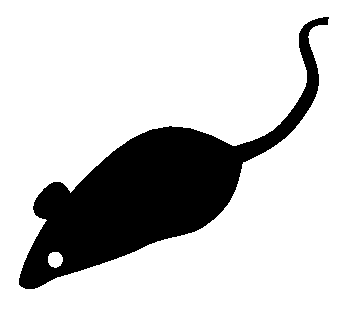
\includegraphics[width=2.25in]{mouse.eps}}
\caption{An example of figure caption. An example of figure
caption. An example of figure caption. An example of figure
caption.}
\label{f:mouse1column}
\end{figure}


At \hbox{100\,$\umu$m} the infrared sky is characterized by emission,
called infrared cirrus, from interstellar dust on all spatial scales
\citep{b16}, thereby impairing the measurements at far-infrared
wavelengths. \eqnbreaktop{3pc} In Figure~\ref{f:shortmouse}, we have plotted the
[60]--[100] colors of the six RV Tauri stars detected at
\hbox{100\,$\umu$m} against their [25]--[60] colors, along with the
grid showing the regions of different values for inner shell
temperature $T_0$ and the quantity $Q$, as in Figure~\ref{f:bigmouse}.
The results indicated by Figure~\ref{f:shortmouse} are consistent with
those derived from Figure~\ref{f:mouse1column}.  AR Pup shows a large
excess at \hbox{100\,$\umu$m} but, in view of the large values for the
cirrus flags given in the catalog, the intrinsic flux at
\hbox{100\,$\umu$m} is uncertain.


\subsection{Radial Distribution of Dust}


From Figure~\ref{f:shortmouse}, it is evident that all RV Tauri stars
lie between the lines corresponding to $Q=1.5$ and 0.5. With
 \[
  \alpha=-(1+Q)\beta-3,
 \]
 these values suggest limits of $r^{-2.0}$ and $r^{-2.4}$ for the dust
density variation, indicating a near-constant mass-loss rate.
\citet{b12} has suggested that the density in the circumstellar
envelope around RV Tauri stars varies as $r^{-1}$, implying a
mass-loss rate that was greater in the past than it is currently.  By
fitting a power law to the observed fluxes, such that $f(\nu)$ varies
as $\nu^q$, values of $q$ determined by him for the various objects
given in Table~\ref{t:tableone} lie in the range 0.6--1.2, with a mean
$\skew5\bar q=0.98$. The assumption of a power law corresponds to the
case of $X_0=0$ in equation (3) and hence we get
 \[
  q=2+\gamma -Q.
 \]
Since we assume that $Q_{\rmn{abs}}(\nu)$ varies as $\nu$, the
resulting value for $Q$=2.0. None of the objects is found to lie in the
corresponding region in the color--color diagram. Even this extreme
value for $Q$ implies a density which varies as $r^{-1.8}$.

\citet{b9} have reported that the simultaneous optical and near-IR
data of AC Her can be fitted by a combination of two blackbodies
at 5680 and 1800\,K, representing, respectively, the stellar and
dust shell temperatures, and suggested that in RV Tauri stars the
grain formation is a sporadic phenomenon and not a continuous
process. Apparently, they have been influenced by the remark by
\citet{b7} that their data in the 3.5--11$\,\umu$m region of AC
Her indicated a dust temperature of $\sim$300\,K. We find that the
{\it K--L\/} colors given by \citet{b5} and
\citet{b9} are all consistent with each other. Surely, hot dust
($\sim$1800\,K), if present at the time of observations by
\citet{b9}, would have affected the {\it K--L\/} color
significantly. AC Her, like other members of its class, is found
to execute elongated loops in the ({\it U--B\/}), ({\it B--V\/})
plane \citep{b20}, indicating that significant departure of the
stellar continuum from the blackbody is to be expected. Further,
their data show only a marginal excess at the near-IR wavelengths.\vspace*{-4pt}
\begin{enumerate}
\item[{\it Step} 1:] The attenuated and diluted stellar radiation;
\item[{\it Step} 2:] Scattered radiation, and
\item[{\it Step} 3:] Reradiation from other grains.\vspace*{-8pt}
\end{enumerate}


\enlargethispage{-2pt}

\subsection{An Example of Head two}
\subsubsection{An example of head three comparison with oxygen and~carbon~Miras}

In Figure~\ref{f:shortmouse} we have also shown the positions of a
sample of oxygen-rich and carbon-rich Miras.  We feel that the case
for the existence of hot dust around AC Her and hence for the sporadic
grain formation around RV Tauri stars is not strong. In
Figure~\ref{f:bigmouse}, we find that AC Her and RU Cen lie very close
to R Sct which, according to \citet{b9}, shows no evidence for the
presence of a hot dust envelope. At the low temperatures
characteristic of the Miras, a part of the emission at 12$\,\umu$m
comes from the photosphere.  For a blackbody at 2000$\,$K, the ratio
of fluxes at wavelengths of 12 and 2$\,\umu$m $(f_{12}/f_{2})\sim
0.18$. The Miras shown in Figure~\ref{f:bigmouse} have
$(f_{12}/f_{2})$ ratios larger than twice the above value. It is clear
that the three groups of objects populate three different regions of
the diagram. \citet{b10} have already noticed that there are distinct
differences between the {\it NIFT\/} colors of oxygen-rich and
carbon-rich objects. On the basis of an analysis, using a bigger
sample of bright giant stars in the {\it NIFT\/} catalog, this has
been interpreted by \citet{b25} as being due to a systematic
difference in the dust grain emissivity index.

\begin{figure*}
  \centerline{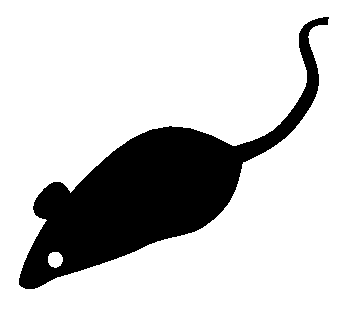
\includegraphics[width=4.5in]{mouse.eps}}
  \caption{An example of figure caption. An example of 
  figure caption. An example of figure caption. An example of
   figure caption. An example of figure caption.}
\label{f:bigmouse}
\end{figure*}

\looseness-1U Mon shows the 10-$\umu$m silicate emission convincingly and, in
most of the other objects for which low-resolution spectra in the
near-infrared have been reported \citep{b5,b19}, the 10-$\umu$m
emission may be partly attributed to silicates. Hence it is
reasonable to expect that, in the envelopes around at least some
of the RV Tauri stars, the dust grains are predominantly of
silicates, as in the case of oxygen Miras \citep{b21}. The fact
that none of the RV Tauri stars is found in the region of the
two-color diagram occupied by the oxygen Miras indicates that the
emissivity indices of the silicate grains in the two cases are
different. Because of the higher temperatures and luminosities,
the environment of grain formation will be different in RV Tauri
stars.
\begin{figure}[b]
  \centerline{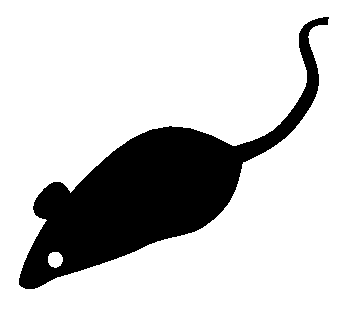
\includegraphics[width=2in]{mouse.eps}}
  \caption{An example of short figure caption.}
\vspace*{-3pt}
\label{f:shortmouse}
\end{figure}

\paragraph{Correlation with subgroups}%
\citet{b20} have identified three spectroscopic subgroups, which
are designated as groups A, B and C. Objects of group A are
metal-rich; group C are metal-poor; group B objects are also
metal-poor, but  show carbon enhancements \citep{b20,b14,b4,b1}.\vspace*{-6pt}
\begin{theorem}
It is interesting to see that Table~\ref{t:tableone} contains no group
C objects and that in Figure~\ref{f:shortmouse} there is a clear
separation of the two spectroscopic subgroups A and B, with the
demarcation occurring at an inner shell temperature of about 450$\,$K,
group B stars having lower temperatures than group A.
\end{theorem}
\begin{proof}
It is interesting to see that Table~\ref{t:tableone} contains no group
C objects and that in Figure~\ref{f:shortmouse} there is a clear
separation of the two spectroscopic subgroups A and B, with the
demarcation occurring at an inner shell temperature of about 450$\,$K,
group B stars having lower temperatures than group A.
\end{proof}
It is interesting to see that Table~\ref{t:tableone} contains no group
C objects and that in Figure~\ref{f:shortmouse} there is a clear
separation of the two spectroscopic subgroups A and B, with the
demarcation occurring at an inner shell temperature of about 450$\,$K,
group B stars having lower temperatures than group A. SX Cen is the
only exception. \citet{b14} has reported that metal lines are stronger
in SX Cen than in other group B objects. It may be worth noting that
SX Cen has the shortest period among the 100 or so objects with the RV
Tauri classification. RU Cen has the coolest inner shell temperature,
as already suggested by the near-infrared spectrum\break \citep{b6}.

\begin{sidewaystable}
 \centering
 \def\~{\hphantom{0}}
% \begin{minipage}{225mm}
  \hsize\textheight
  \caption{It is for us, the living, rather to be
dedicated here to the unfinished work which, so nobly
carried out}
\label{t:sidetable}
\hskip-12pt\begin{tabular*}{\textheight}{@{}l@{\extracolsep{\fill}}c@{\extracolsep{\fill}}r@{\extracolsep{\fill}}r@{\extracolsep{\fill}}r@{\extracolsep{\fill}}r@{\extracolsep{\fill}}l@{\extracolsep{\fill}}c@{\extracolsep{\fill}}c@{\extracolsep{\fill}}c@{\hskip12pt}}
  \Hline
 & & \multicolumn{4}{c}{{Flux density (Jy)} \footnote{Observed by {\em NIFT}.}}\\ [1pt]
\cline{3-7} \\ [-6pt]
{Name}        &  & & & & & {Sp.} & \multicolumn{1}{r}{Period}& \multicolumn{1}{l}{Light-} 		\\ [-3pt]
{Variable}\footnote{Observed by {\em NIFT}.}        &
{\it NIFT} & {12$\,\umu$m} & {25$\,\umu$m} & {60$\,\umu$m}
     & {100$\,\umu$m} &     {group} & \multicolumn{1}{r}{(d)}    &
	 \multicolumn{1}{l}{curve type}& {\em T$_0$\,(\rm{K})}  \\ 
 \hline
 TW Cam & 04166$+$5719 & 8.27   & 5.62 & 1.82  & $<$1.73   & A & \~85.6 & a & 555 \\
 CT Ori & 06072$+$0953 & 6.16   & 5.57 & 1.22  & $<$1.54   & B & 135.6 &  & 330 \\
 SU Gem & 06108$+$2734 & 7.90   & 5.69 & 2.16  & $<$11.66  & A & \~50.1 & b & 575 \\
 UY CMa & 06160$-$1701 & 3.51   & 2.48 & 0.57  & $<$1.00   & B & 113.9 & a & 420 \\
 U Mon  & 07284$-$0940 & 124.30 & 88.43& 26.28 & 9.24      & A & \~92.3 & b & 480 \\
 AR Pup & 08011$-$3627 & 131.33 & 94.32& 25.81 & 11.65     & B & \~75.0 & b & 450 \\
 IW Car & 09256$-$6324 & 101/06 & 96.24& 34.19 & 13.07     & B & \~67.5 & b & 395 \\
 RU Cen & 12067$-$4508 & 5.36   & 11.02& 5.57  & 2.01      & B & \~64.7 &  & 255 \\
 SX Cen & 12185$-$4856 & 5.95   & 3.62 & 1.09  & $<$1.50   & B & \~32.9 & b & 590 \\
 AI Sco & 17530$-$3348 & 17.68  & 11.46& 2.88  & $<$45.62  & A & \~71.0 & b & 480 \\
 AC Her & 18281$+$2149 & 41.47  & 65.33& 21.12 & 7.79      & B & \~75.5 & a & 260 \\
 R Sct  & 18448$-$0545 & 20.88  & 9.30 & 8.10  & $<$138.78 & A & 140.2 & a \\
 R Sge  & 20117$+$1634 & 10.63  & 7.57 & 2.10  & $<$1.66   & A & \~70.6 & b & 455 \\
\hline
\end{tabular*}
%\end{minipage}
\end{sidewaystable}

\subsubsection{Correlation with subgroups}%
\paragraph{Head four correlation with subgroups}%
Group B objects follow a different mean relationship from those of
group A, having systematically larger 11-$\umu$m excess for a given
excess at 3$\,\umu$m. For a general sample of RV Tauri stars, the
distinction between the oxygen-rich and carbon-rich objects is not
that apparent in the {\it JHKL\/} bands. In Figure~\ref{f:shortmouse}
we have plotted the near-IR magnitudes of the objects given in
Table~\ref{t:sidetable} (except V Vul which has no available
measurements) in the {\it J--K, K--L\/} plane. The colors, taken from
\citet{b9}, are averaged if more than one observation exists, because
the internal agreements are found to be often of the order of
observational uncertainties, in accordance with the earlier finding by
\citet{b5} that variability has relatively little effect on
colors. Barring RU Cen and AC Her, it is evident that stars belonging
to group B show systematically larger excebioms at {\it L\/} band for
a given excess at {\it K}. The low excebioms at near-IR wavelengths
for AC Her and RU Cen are consistent with the very low dust
temperatures indicated by the far-infrared colors.
%

It is already well established that from {\it UBV\/} photometry one
can distinguish between groups A and B, members of group A being
significantly redder than those of group B \citep{b20}.  Similarly,
\citet{b4} has found that the two spectroscopic groups are well
separated in the DDO color--color diagrams when mean colors are
used for the individual objects. The clear separation of the
spectroscopic subgroups A and B in the IR two-color diagram suggests
that the natures of dust grains in the envelopes in the two cases are
not identical. This is to be expected because of the differences in
the physical properties of the stars themselves. The average colors
of group B stars are bluer than group A, but the envelope dust
temperatures of B are cooler than those of A. The near-IR spectra of
AC Her and RU Cen are extremely similar \citep{b6}. The striking
similarities in the optical spectra of AC Her and RU Cen have been
pointed out by Bidelman \citep{b18}. We feel that the physical
properties, including the chemical composition, of the grains formed
in the circumstellar envelope strongly depend on those of the embedded
star. This, probably, explains the diversity of the energy
distributions of RV Tauri stars in the near-infrared found by
\citet{b6}. On the basis of the observed differences in chemical
abundances and space distribution of RV Tauri stars {\tt
http://www.duke.edu/$\sim$delon001/Biometrics\_tables.pdf}.  See
Section~\ref{s:discuss} for further discussion.

\citet{b13} have subdivided RV Tauri stars into two clabioms, RVa and
RVb, on the basis of their light curves; the former shows a constant
mean brightness, whereas the latter shows a cyclically varying mean
brightness. Extensive observations in the near-infrared show that, on
average, RVb stars are redder than RVa stars, In RVb stars dust shells
are denser in the inner regions and hence radiate strongly in the
1--3$\,\umu$m region. Figure~\ref{f:shortmouse} confirms this; RVb
objects show systematically larger ({\it J--K\/}) and ({\it K--L\/})
colors than RVa objects. Apparently, there is no distinction between
objects of the two light-curve types at far-infrared wavelengths
(Figure~\ref{f:shortmouse}).

\section{Discussion}
\label{s:discuss}

In the [12]--[25], [25]--[60] color diagram, RV Tauri stars populate
cooler temperature regions $(T<600 \,\rmn{K})$, distinctly different from
those occupied by the oxygen and carbon Miras. Using a simple model
in which
\begin{enumerate}
  \item[1.] the envelope is spherically symmetric,
  \item[2.] the IR-emitting grains are predominantly of the same kind, and
  \item[3.] in the infrared the absorption efficiency $Q_{\rmn{abs}}
        (\nu)\propto\nu$,
\end{enumerate}
we find that the {\it NIFT\/} fluxes are consistent with the
density in the envelope $\rho(r)\propto r^{-2}$, where {\it r\/}
is the radial distance. Such a dependence for the dust density
implies that the mass-loss rates in RV Tauri stars have not
reduced considerably during the recent past, contrary to the
suggestion by \citet{b12}. In the two-color diagram, the
blackbody line and the line corresponding to $\rho(r)\propto
r^{-2.2}$ nearly overlap and the present data are insufficient to
resolve between the two cases. The latter case is more physically
reasonable, however.

\backmatter

%%%%%% include this section if you wish to acknowledge people,
%%%%%% grant support, etc.

\section*{Acknowledgements}

The authors thank Professor A. Sen for some helpful suggestions,
Dr C. R. Rangarajan for a critical reading of the original version of the
paper, and an anonymous referee for very useful comments that improved
the presentation of the paper.\vspace*{-8pt}

%%%%%% include this section only if your manuscript refers to supplementary
%%%%%% materials -- see Instructions for Authors at 
%%%%%% http://www.tibs.org/biometrics

\section*{Supplementary Materials}

Web Appendix 1 referenced in Section~\ref{ss:example} is available
with this paper at the Biometrics website on Wiley Online Library.
\vspace*{-8pt}


\begin{thebibliography}{}
\bibitem[\protect\citeauthoryear{Akash and Tirky}{1988}]{b24} 
Akash, F. J. and Tirky, T. (1988). Proper multivariate conditional
autoregressive models for spatial data analysis. {\it Biometrics} {\bf 196,} 173.

\bibitem[\protect\citeauthoryear{Balaram et~al.}{1985a}]{b2} 
Balaram, C. A., Neeraj, G., Haq, H. J., and Cliff, P. E., (1985a). {\it
NIFT\/} 2nd edition. Boca Raton, Florida: Chapman and Hall.

\bibitem[\protect\citeauthoryear{Commel}{1961}]{b18} 
Commel, J. K. (1961). {\it National Sangget Academia}, 2nd edition.
Hoboken, New Jersey: Wiley.

\bibitem[\protect\citeauthoryear{Das  and Patra}{1986}]{b25} 
Das, B. and Patra, H. M. (1986). Using counts to simultaneously estimate
abundance and detection probabilities in a salamander community. {\it
Herpetologica} {\bf 60,} 468--478.

\bibitem[\protect\citeauthoryear{Emrat}{1974}]{b14} Emrat, T. (1974).
{\it Topics in Stochastic Processes.} New York: Academic  Press.

\bibitem[\protect\citeauthoryear{Emrat}{1985}]{b15} Emrat, T. (1985).
{\it Topics in Stochastic Processes.} New York: Academic  Press.

\bibitem[\protect\citeauthoryear{Goldman et~al.}{1987}]{b9} 
Goldman, M. J. and Ewin, A. (1987). A comparison of smoothing
techniques for CD4 data measured with error in a time-dependent Cox
proportional hazards model. {\it Statistics in Medicine} {\bf 17,} 2061--2077.

\bibitem[\protect\citeauthoryear{Goodsman}{1972}]{b8} 
Goodsman, R. C. (1972). Testing hypotheses in the functional linear
model. {\it Scandinavian Journal of Statistics} {\bf 30,} 241--251.

\bibitem[\protect\citeauthoryear{Gooms}{1972}]{b5} Gooms, R. D.
(1972). Goodsman, R.C. (1972). Testing hypotheses in the functional linear
model. {\it Scandinavian Journal of Statistics} {\bf 31,} 315--323.


\bibitem[\protect\citeauthoryear{Gooms  and Wool}{1970}]{b7} Gooms,
R. D. and Wool, N. J. (1970). A comparison of smoothing
techniques for CD4 data measured with errors in a time-dependent Cox
proportional hazards model. {\it Statistics in Medicine} {\bf 17,} 2091--2099.

\bibitem[\protect\citeauthoryear{Hackel}{1985}]{b10} 
Hackel, P. (1985). {\it Topics in Stochastic Processes.} New York: Academic  Press.

\bibitem[\protect\citeauthoryear{\nobreak Holloman, \nobreak Tinku,  and Gerg}{Holloman et~al.}{1979}]{b11}
Holloman, P. M., Tinku, H. A., and Gerg, I. (1979). A comparison of smoothing
techniques for CD4 data measured with techniques a time-dependent Cox
proportional hazards model. {\it Statistics in Medicine} {\bf 17,} 2105--2111.

\bibitem[\protect\citeauthoryear{Juman}{1986}]{b12} 
Juman, M. (1986). Using counts to simultaneously estimate
abundance and detection probabilities in a salamander community. {\it
Herpetologica} {\bf 61,} 482--495.

\bibitem[\protect\citeauthoryear{Kartik B}{1969}]{b13} 
Kartik, B. V. (1969). Using counts to simultaneously estimate
abundance and detection probabilities in a salamander community. {\it
Herpetologica} {\bf 62,} 511--519.

\bibitem[\protect\citeauthoryear{Lenin}{1932}]{b17} 
Lenin, D. B. (1932). A comparison of smoothing
techniques for CD4 data measured with errors in a time-dependent Cox
proportional hazards model. {\it Statistics in Medicine} {\bf 17,} 2125--2135.

\bibitem[\protect\citeauthoryear{O'Rourke}{1979}]{b4} O'Rourke, D. (1996). Industrial ecology: A 
critical review. {\it International Journal of Environment and Pollution}
{\bf 6,} 389--112.

\bibitem[\protect\citeauthoryear{Oman and \nobreak Raj}{1986}]{b19}
Oman, F. M. and  Raj, E. (1986). {\it Topics in Stochastic Process.} New York: Academic  Press.

\bibitem[\protect\citeauthoryear{Prem et~al.}{1963}]{b20} Prem, G. W., Christ, W., Smap, J.,
Wills, J. A. (1963). {\it Topics in Stochastic Processes.} New York: Academic  Press.

\bibitem[\protect\citeauthoryear{Rahul}{1981}]{b1} Rahul, S. R. (1981).
Industrial ecology: A  critical review. {\it International Journal of
Environment and Pollution} {\bf 6,} 371--375.

\bibitem[\protect\citeauthoryear{Ram  and Shyam}{1972}]{b6} Ram, R. D.
and Shyam, S. (1972). {\it Topics in Stochastic Process.} New York: Academic  Press.

\bibitem[\protect\citeauthoryear{Ravan  and Hari}{1983a}]{b21} Ravan,
M. and Hari, S. (1983). Industrial ecology: A  critical review.
{\it International Journal of Environment and Pollution} {\bf 6,} 389--395.

\bibitem[\protect\citeauthoryear{Ravan  and Hari}{1983b}]{b22}
Ravan, M. and Hari, S. (1984). Industrial ecology: A  critical
review. {\it International Journal of Environment and Pollution} {\bf 7,} 512--519.

\bibitem[\protect\citeauthoryear{Sharma et~al.}{1984}]{b16} Sharma,
F. J. (1984). {\it Topics in Stochastic Process.} New York: Academic Press.

\bibitem[\protect\citeauthoryear{Vim   and Potter}{1988}]{b23} Vim, W.
E. and Potter, H. J. (1988). A  critical
review. {\it International Journal of Environment and Pollution} {\bf 9,} 635--641.

\end{thebibliography}

\appendix

\section{}
\subsection{Computation of E$_i\{\alpha_i\}$}

(This appendix was not part of the original paper by
A.V.~Raveendran and is included here just for illustrative
purposes. The references are not relevant to the text of the
appendix, they are references from the bibliography used to
illustrate text before and after citations.)

Here is an equation; note how it is numbered:
\begin{equation}
A = B+C. 
\label{eq:appeq}
\end{equation}
Equation~(\ref{eq:appeq}) is an the only numbered equation in this appendix.

Spectroscopic observations of bright quasars show that the mean
number density of Ly$\alpha$ forest lines, which satisfy certain
criteria, evolves like $\rmn{d}N/\rmn{d}z=A(1+z)^\gamma$, where
$A$ and~$\gamma$ are two constants.  Given the above intrinsic
line distribution we examine the probability of finding large gaps
in the Ly$\alpha$ forests.  We concentrate here only on the
statistics and neglect all observational complications such as the
line blending effect \citep[see][for example]{b11}. We concentrate here only on the
statistics and neglect all observational complications such as the
line blending effect \citep[see][for example]{b11}. We concentrate here only on the
statistics and neglect all observational complications such as the
line blending effect \citep[see][for example]{b11}. 

The references are not relevant to the text of the
appendix, they are references from the bibliography used to
illustrate text before and after citations.)

Spectroscopic observations of bright quasars show that the mean
number density of Ly$\alpha$ forest lines, which satisfy certain
criteria, evolves like $\rmn{d}N/\rmn{d}z=A(1+z)^\gamma$, where
$A$ and~$\gamma$ are two constants.  Given the above intrinsic
line distribution we examine the probability of finding large gaps
in the Ly$\alpha$ forests.  We concentrate here only on the
statistics and neglect all observational complications such as the
line blending effect \citep[see][for example]{b11}. We concentrate here only on the
statistics and neglect all observational complications such as the
line blending effect \citep[see][for example]{b11}. We concentrate here only on the
statistics and neglect all observational complications such as the
line blending effect \citep[see][for example]{b11}. \vadjust{\vfill\pagebreak}

Suppose we have observed a Ly$\alpha$ forest between redshifts $z_1$
and~$z_2$ and found $N-1$ lines.  For high-redshift quasars $z_2$~is
usually the emission redshift $z_{\rmn{em}}$ and $z_1$ is set to
$(\lambda_{\rmn{Ly}\beta}/\lambda_{\rmn{Ly}\alpha})(1+z_{\rmn{em}})=0.844
(1+z_{\rmn{em}})$ to avoid contamination by Ly$\beta$ lines.  We
want to know whether the largest gaps observed in the forest are
significantly inconsistent with the above line distribution.  To do
this we introduce a new variable~$x$:\vspace*{1.5pt}
%
\[
x={(1+z)^{\gamma+1}-(1+z_1)^{\gamma+1} \over
     (1+z_2)^{\gamma+1}-(1+z_1)^{\gamma+1}}.
\]
\vskip1.5pt%
$x$ varies from 0 to 1.  We then have $\rmn{d}N/\rmn{d}x=\lambda$,
where $\lambda$ is the mean number of lines between $z_1$ and $z_2$
and is given by
%
\[%
\lambda\equiv{A[(1+z_2)^{\gamma+1}-(1+z_1)^{\gamma+1}]\over\gamma+1}.
\]
%
This means that the Ly$\alpha$ forest lines are uniformly
distributed in~$x$.
%
\label{lastpage}

\end{document}
